%
% This is the LaTeX template file for lecture notes for EE 382C/EE 361C.
%
% To familiarize yourself with this template, the body contains
% some examples of its use.  Look them over.  Then you can
% run LaTeX on this file.  After you have LaTeXed this file then
% you can look over the result either by printing it out with
% dvips or using xdvi.
%
% This template is based on the template for Prof. Sinclair's CS 270.

\documentclass[twoside]{article}
\usepackage{graphics}
\setlength{\oddsidemargin}{0.25 in}
\setlength{\evensidemargin}{-0.25 in}
\setlength{\topmargin}{-0.6 in}
\setlength{\textwidth}{6.5 in}
\setlength{\textheight}{8.5 in}
\setlength{\headsep}{0.75 in}
\setlength{\parindent}{0 in}
\setlength{\parskip}{0.1 in}

%
% The following commands set up the lecnum (lecture number)
% counter and make various numbering schemes work relative
% to the lecture number.
%
\newcounter{lecnum}
\renewcommand{\thepage}{\thelecnum-\arabic{page}}
\renewcommand{\thesection}{\thelecnum.\arabic{section}}
\renewcommand{\theequation}{\thelecnum.\arabic{equation}}
\renewcommand{\thefigure}{\thelecnum.\arabic{figure}}
\renewcommand{\thetable}{\thelecnum.\arabic{table}}

%
% The following macro is used to generate the header.
%
\newcommand{\lecture}[4]{
   \pagestyle{myheadings}
   \thispagestyle{plain}
   \newpage
   \setcounter{lecnum}{#1}
   \setcounter{page}{1}
   \noindent
   \begin{center}
   \framebox{
      \vbox{\vspace{2mm}
    \hbox to 6.28in { {\bf EE 382C/361C: Multicore Computing
                        \hfill Fall 2016} }
       \vspace{4mm}
       \hbox to 6.28in { {\Large \hfill Lecture #1: #2  \hfill} }
       \vspace{2mm}
       \hbox to 6.28in { {\it Lecturer: #3 \hfill Scribe: #4} }
      \vspace{2mm}}
   }
   \end{center}
   \markboth{Lecture #1: #2}{Lecture #1: #2}
   %{\bf Disclaimer}: {\it These notes have not been subjected to the
   %usual scrutiny reserved for formal publications.  They may be distributed
   %outside this class only with the permission of the Instructor.}
   \vspace*{4mm}
}

%
% Convention for citations is authors' initials followed by the year.
% For example, to cite a paper by Leighton and Maggs you would type
% \cite{LM89}, and to cite a paper by Strassen you would type \cite{S69}.
% (To avoid bibliography problems, for now we redefine the \cite command.)
% Also commands that create a suitable format for the reference list.
\renewcommand{\cite}[1]{[#1]}
\def\beginrefs{\begin{list}%
        {[\arabic{equation}]}{\usecounter{equation}
         \setlength{\leftmargin}{2.0truecm}\setlength{\labelsep}{0.4truecm}%
         \setlength{\labelwidth}{1.6truecm}}}
\def\endrefs{\end{list}}
\def\bibentry#1{\item[\hbox{[#1]}]}

%Use this command for a figure; it puts a figure in wherever you want it.
%usage: \fig{NUMBER}{SPACE-IN-INCHES}{CAPTION}
\newcommand{\fig}[3]{
			\vspace{#2}
			\begin{center}
			Figure \thelecnum.#1:~#3
			\end{center}
	}
% Use these for theorems, lemmas, proofs, etc.
\newtheorem{theorem}{Theorem}[lecnum]
\newtheorem{lemma}[theorem]{Lemma}
\newtheorem{proposition}[theorem]{Proposition}
\newtheorem{claim}[theorem]{Claim}
\newtheorem{corollary}[theorem]{Corollary}
\newtheorem{definition}[theorem]{Definition}
\newenvironment{proof}{{\bf Proof:}}{\hfill\rule{2mm}{2mm}}

% **** IF YOU WANT TO DEFINE ADDITIONAL MACROS FOR YOURSELF, PUT THEM HERE:
\usepackage{graphicx}
\graphicspath{ {images/} }

\begin{document}
%FILL IN THE RIGHT INFO.
%\lecture{**LECTURE-NUMBER**}{**DATE**}{**LECTURER**}{**SCRIBE**}
\lecture{11}{September 29}{Vijay Garg}{William Mills}
%\footnotetext{These notes are partially based on those of Nigel Mansell.}

% **** YOUR NOTES GO HERE:

% Some general latex examples and examples making use of the
% macros follow.  
%**** IN GENERAL, BE BRIEF. LONG SCRIBE NOTES, NO MATTER HOW WELL WRITTEN,
%**** ARE NEVER READ BY ANYBODY.
\section{Exam 1 Study Tips}
Exam 1 will only cover up-through Lecture 11 (today)
There will be a problem from the seminar
Some sample problems have been posted on Canvas. It is advised that you follow this order in your studying:
\begin{enumerate}
\item Attempt the problems on your own
\item Compare your solutions with your peers 
\item Solutions will be posted next week to check for correctness
\end{enumerate}
Additionally, Homework 3 has been posted, and some of its questions will be good preparation (but some of it has not been covered yet)
The material to best-prepare you, in descending order:
\begin{enumerate}
\item Material covered in both Lecture and Handouts
\item Material covered in Lecture only
\item Material covered in Handouts only
\item Past Assignments
\end{enumerate}

\newpage

\section{Concurrent History Equivalence}

Recall that a concurrent History $(H, <_H)$ is a sequential history $(S, <_S)$ if $<_S$ is a total order.
Two histories are {\em equivalent} if they are composed of the same operations.

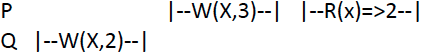
\includegraphics{H1}
\fig{1}{2px}{H1}

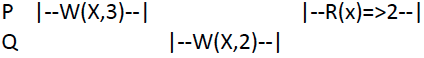
\includegraphics{H2}
\fig{2}{2px}{H2}

Observe that {\tt H2} is simply a permutation of the operations in {\tt H1}, but {\tt H1} is not identical to {\tt H2}. These two histories are equivalent.
\section{Sequential Consistency}

A history $(H, <_H)$ is {\em sequentially consistent} if there exists a legal sequential history {\tt S} such that:
\begin{enumerate}
\item {\tt S} is equivalent to {\tt H}
\item {\tt S} preserves the process order in $(H, <_H)$
\end{enumerate}

Both {\tt H1} and {\tt H2} from the previous section are sequentially consistent. A legal sequential history for either of them would be

$P: W(X,3), Q: W(X,2), P: R(X)=>2$

Now consider History {\tt H3}:

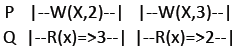
\includegraphics{H3}
\fig{3}{2px}{H3}

\newpage

{\tt H3} is NOT sequentially consistent. This can be shown by adding arrows that represent the {\em happened-before} relationship. When a cycle is identified, we know the history is not legal and thus cannot be sequentially consistent. When we place these edges in {\tt H3}, we can see that a cycle exists when we follow the {\em happened-before} relationship:

$P: W(X,2), \underline{Q: R(X)=>2, P W(X,3), Q: R(X)=>3, Q: R(X)=>2}$

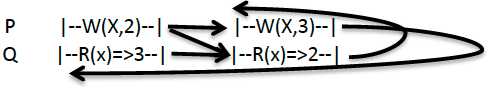
\includegraphics{H3WLines}
\fig{4}{2px}{H3}

\section{Atomic Consistency (Linearization)}

A history $(H, <_H)$ is linearizable/atomically consistent if there exists a legal sequential history {\tt S} such that
\begin{enumerate}
\item {\tt S} is equivalent to {\tt H}
\item {\tt S} preserves $<_H$
\begin{itemize}
\item That is, responses occurring before invocations in {\tt H} must preserve that relationship in {\tt S}
\end{itemize}
\end{enumerate}

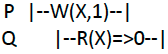
\includegraphics{H4}
\fig{5}{2px}{H4}

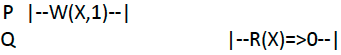
\includegraphics{H5}
\fig{6}{2px}{H5}

Thus, {\tt H4} is linearizable, while {\tt H5} is not.

\subsection{Linearization Points}

To help determine if a history is linearizable, We can think of each operation having a single moment where its effect takes place, and try to find an order for them. We call such moments {\em linearization points}.
Theorem: {\tt H} is linearizable if there exist linearization points for all operations such that the resulting sequence is legal.

\section{Composability (Locality Property)}

Linearization is arguably a better tool for software applications, because it has the {\em locality property}, which says the concurrent history is legal when multiple objects are considered.

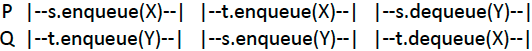
\includegraphics{H7}
\fig{7}{2px}{H7}

Note that {\tt H7} is linearizable when all of object $t$'s operations are ignored. The same holds when all of $s$'s operations are ignored. However, when the two are combined, we see that there is a cycle the same way we did before.

$P: s.enqueue(X), t.enqueue(X), t.enqueue(Y), s.enqueue(Y), s.enqueue(X)$

When a history {\tt H} is projected on an object $x$, we write the sub-history as $H|x$. Note that $H|s$ and $H|t$ are both sequentially consistent, but {\tt H} is not, because there is a cycle in its $<_H$ trace.

\subsection{Linearization and the Locality Property}
By definition, a consistency condition {\tt CONSISTENCY} satisfies composability if:

$\forall x, H|x satisfies {\tt CONSISTENCY} \Leftrightarrow H satisfies {\tt CONSISTENCY}$

Linearizability can be shown to satisfy composability from this definition. It is trivial to show that $H is linearizable \rightarrow \forall x, H|x is linearizable$, so we will focus on the proof for the other direction.

As before, we will place arrows on our history to represent the happened-before relation. The claim is that adding these arrows will maintain an acyclic representation of the history. These arrows can be drawn for two reasons:
\begin{enumerate}
\item $<_H$ enforces it
\item $<_x \forall x$
\end{enumerate}

We know arrows from {\tt 1} cannot form a cycle because they are enforced by the poset they come from. It remains to be shown that traces including both types of arrows cannot introduce a cycle. We assert that such subpaths including {\tt 1} $\rightarrow$ {\tt 2} $\rightarrow$ {\tt 1} can be re-written as a single arrow of type {\tt 1}.

$e <_H f$ -- response($e$) happened before invocation($f$).
$f <_x g$ -- response($e$) happened before invocation($f$).
$g <_H h$ -- response($e$) happened before invocation($f$).

Transitively, we know that $c <_H h$ holds.

\section{All Concurrent Histories}

There are many other types of histories looser than sequential consistency that we did not discuss. Realize that the weaker your consistency rules are, the better performance you can achieve with the same hardware.

For this class, we will stick to atomic consistency

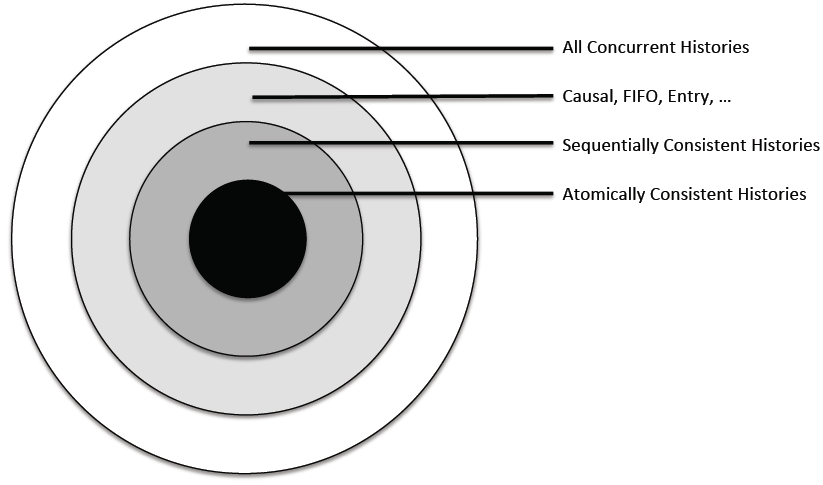
\includegraphics[scale=0.5]{historySubsumption.png}
\fig{7}{2px}{Concurrent History Strengths}

\section*{References}
\beginrefs
\bibentry{1}{\sc V. K. Garg}, Introduction to Multicore Computing
\endrefs


\end{document}





